\documentclass[tikz,border=2pt]{standalone}
\usepackage{amsmath}
\usepackage{pgfplots}
\pgfplotsset{compat=1.18}
\usetikzlibrary{arrows.meta}
\begin{document}
% Used-car example: buyer's expected payoff from offer p is 0 for p<4, 0.6(6-p) for 4<=p<10
% (only L accepts) and 8.4-p for p>=10 (both accept); the maximum is 1.2 at p=4.
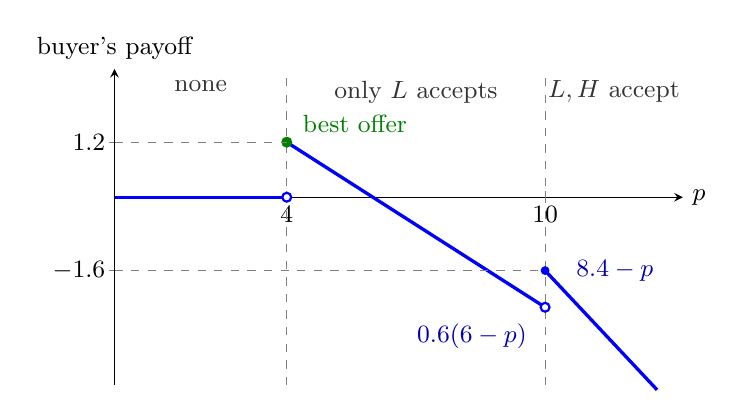
\begin{tikzpicture}[font=\small, >={Latex[length=2mm]}]
  \begin{axis}[
    axis lines=middle,
    xmin=0, xmax=13.2, ymin=-4.1, ymax=2.8,
    xtick={4,10}, ytick={-1.6,1.2},
    yticklabels={$-1.6$,$1.2$},
    xlabel={$p$}, ylabel={buyer's payoff},
    xlabel style={anchor=west}, ylabel style={anchor=south},
    tick label style={font=\small},
    every tick label/.append style={fill=white, inner sep=1pt},
    samples=2, clip=false,
    width=8.8cm, height=5.6cm]
    % seller values (thresholds)
    \draw[gray, dashed, thin] (axis cs:4,-4.1) -- (axis cs:4,2.6);
    \draw[gray, dashed, thin] (axis cs:10,-4.1) -- (axis cs:10,2.6);
    \node[gray!40!black, anchor=north] at (axis cs:2,2.75) {none};
    \node[gray!40!black, anchor=north] at (axis cs:7,2.75) {only $L$ accepts};
    \node[gray!40!black, anchor=north] at (axis cs:11.6,2.75) {$L,H$ accept};
    % payoff curve
    \addplot[blue, very thick, domain=0:4] {0};
    \addplot[blue, very thick, domain=4:10] {0.6*(6-x)};
    \addplot[blue, very thick, domain=10:12.6] {8.4-x};
    \draw[blue, thick, fill=white] (axis cs:4,0) circle (1.6pt);
    \draw[blue, thick, fill=white] (axis cs:10,-2.4) circle (1.6pt);
    \fill[blue] (axis cs:10,-1.6) circle (1.6pt);
    \fill[green!50!black] (axis cs:4,1.2) circle (2pt);
    \draw[gray, thin, dashed] (axis cs:0,1.2) -- (axis cs:4,1.2);
    \draw[gray, thin, dashed] (axis cs:0,-1.6) -- (axis cs:10,-1.6);
    \node[green!50!black, anchor=south west] at (axis cs:4.15,1.2) {best offer};
    \node[blue!70!black, anchor=north east] at (axis cs:9.8,-2.55) {$0.6(6-p)$};
    \node[blue!70!black, anchor=west] at (axis cs:10.5,-1.6) {$8.4-p$};
  \end{axis}
\end{tikzpicture}
\end{document}
